\chapter{Phân tích thiết kế hệ thống}
\section{Khảo sát hiện trạng của hệ thống}
%Giới thiệu về Nam Hải
Nam Hải là một cửa hàng bán linh kiện có địa chỉ tại 030, đường Hoàng liên, đoạn gần ngân hàng Viettinbank, phường Kim Tân, Thành phố Lào Cai, với quy mô nhỏ, chỉ một người quản lý mảng kinh doanh và một người quản lý mảng buôn bán, nhập hàng.\par
% Tại sao lại tạo website
nhằm mục đích mở rộng thị trường, tiếp cận khách hàng tiềm năng và tạo thương hiệu trên mạng internet, tôi quyết định xây dựng website bán hàng với mặt hàng là các loại linh kiện điện tử (Vi điều khiển, cảm biến, IC, ...) với đối tượng khách hàng hướng tới là những người có đam mê với điện tử, sinh viên các trường công nghệ, ....\par
% Yêu cầu ...
Qua trao đổi với chủ của hàng, trang web cần phải có giao diện dễ nhìn, cho phép khách hàng xem các mặt hàng một cách nhanh chóng, có thể tìm kiếm mặt hàng một cách dễ dàng, về chức năng:
\begin{itemize}
\itemsep0em
\item \textbf{Đối với người dùng:}
    \begin{itemize}
    \item Người dùng chưa đăng nhập được coi là khách hàng.
    \item Khách hàng có thể xem thông tin của sản phẩm (Tên, giá tiền, thông tin chi tiết).
    \item Khách hàng có thể thêm sản phẩm vào giỏ hàng cũng như xóa sản phẩm trong giỏ hàng tuy nhiên để tạo đơn hàng Khách hàng cần đăng nhập vào hệ thống.
    \item Khách hàng sau khi đăng nhập (Nếu chưa có tài khoản Khách hàng cần đăng ký trước) được coi là Người dùng.
    \item Người dùng có thể xem thông tin về những đơn hàng trước đây.
    \item Người dùng có thể cập nhật lại thông tin cá nhân.
    \end{itemize}
\vspace{1em}
\item \textbf{Đối với chủ cửa hàng:}
\itemsep0em
    \begin{itemize}
    \item Để thực hiện các chức năng quản trị Chủ cửa hàng cần đăng nhập bằng tài khoản được lập trình viên cấp.
    \item Sau khi đăng nhập chủ cửa hàng có thể chọn thống kê doanh thu, quản lý sản phẩm, quản lý đơn hàng.
    \item Với chức năng thống kê chủ cửa hàng có thể xem được thống kê về doanh thu, thống kê hàng tồn kho.
    \item Với chức năng quản lý sản phẩm, chủ cửa hàng có thể nhập sản phẩm, cập nhật thông tin sản phẩm, chuyển trạng thái sản phẩm từ kinh doanh sang ngừng kinh doanh và ngược lại.
    \item Với chức năng quản lý đơn hàng, chủ cửa hàng có thể xem được danh sách các đơn hàng chưa được xử lý cũng như các đơn hàng đã xử lý, chủ cửa hàng cũng có thể chuyển trạng thái đơn hàng từ đang tiếp nhận xong đã giao hàng thành công để chuyển đơn hàng sang danh sách đã xử lý.

    \end{itemize}
\end{itemize}

Từ những yêu cầu trên có thể thấy hệ thống cần thực hiện một số chức năng chính như:
\begin{itemize}
\itemsep0em
\item Phân quyền người dùng (Đăng ký, đăng nhập, đăng xuất)
\item Quản lý đơn hàng (xem thông tin đơn hàng, đổi trạng thái đơn hàng)
\item Quản lý sản phẩm (xem và cập nhật thông tin sản phẩm, thay đổi trạng thái sản phẩm)
\item Thống kê (Doanh thu, hàng tồn kho)
\end{itemize}

Ngoài ra hệ thống cũng cần đáp ứng một số yêu cầu phi chức năng khác như: giao diện dễ nhìn, tìm kiếm và xem thông tin sản phẩm nhanh chóng, thuận tiện. Những yêu cầu trên sẽ được xây dựng và hiệu chỉnh theo yêu cầu từ phía chủ cửa hàng để ra.
\section{Phân tích và thiết kế hệ thống}
\subsection{Biểu đồ Usercase}
\begin{enumerate}[label=\textbf{\alph*)}]
\item \textbf{Biểu đồ tổng quát}
    \begin{figure}[h!]
        \centering
        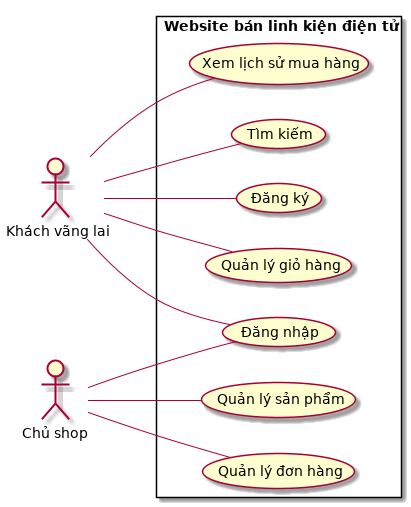
\includegraphics[scale=0.7]{fig/uc_all.png}
        \caption{Biểu đồ tổng quát}
    \end{figure}
\newpage
\item \textbf{Biểu đồ phân rã cho tác nhân Khách hàng}
    \begin{figure}[h!]
        \centering
        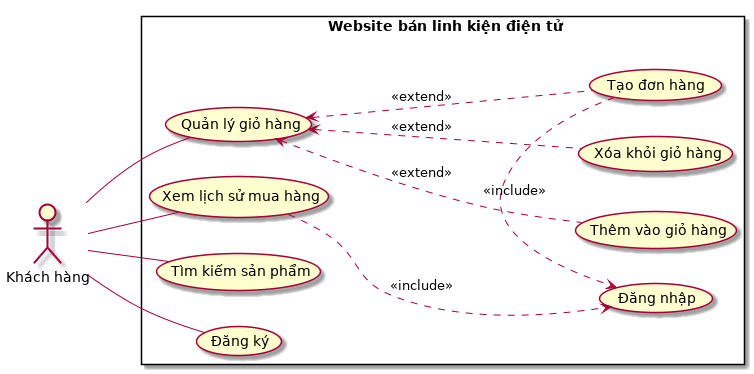
\includegraphics[scale=0.6]{fig/uc_user.png}
        \caption{Biểu đồ phân rã tác nhân Khách hàng}
    \end{figure}
\newpage
\item \textbf{Biểu đồ phân rã cho tác nhân Chủ shop}
    \begin{figure}[h!]
        \centering
        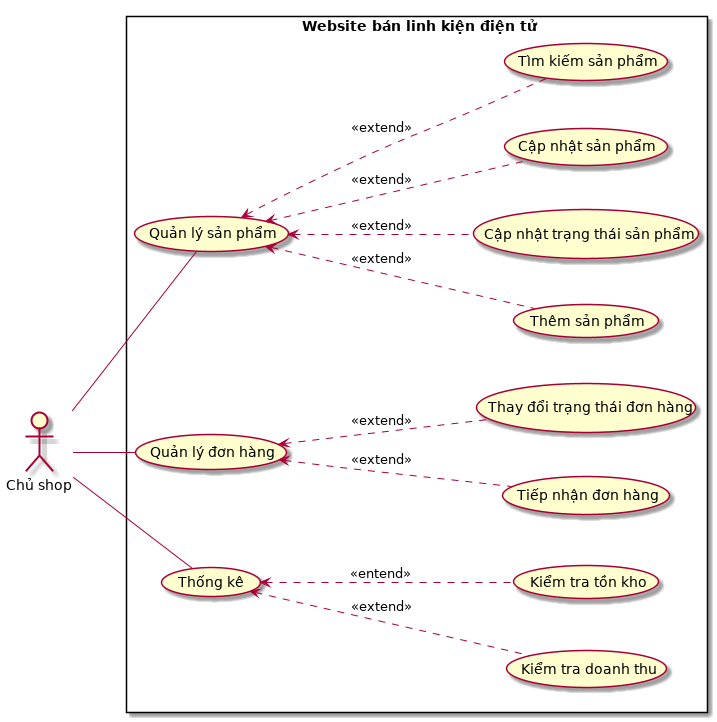
\includegraphics[scale=0.6]{fig/uc_admin.png}
        \caption{Biểu đồ phân rã tác nhân Chủ shop}
    \end{figure}
\end{enumerate}
\subsection{Kịch bản cho một số use case chính}
\begin{center}
\begin{tabularx}{\linewidth}{|X|}
\cline{1-2}
    \textbf{Tên use case:} Quản lý đơn hàng\\
    \textbf{Tác nhân chính:} Chủ shop\\
    \textbf{Mức:} 1\\
    \textbf{Tiền điều kiện:} Người dùng cần đăng nhập và tài khoản dùng để đăng nhập có quyền quản trị\\
    \textbf{Luồng kịch bản chính:}\\
    \begin{enumerate}
        \vspace{-2em}
        \itemsep-0.5em
        \item Chủ shop cần abc
        \item Chủ shop bcd
        \item Chủ shop XYZ
        \vspace{-1em}
    \end{enumerate}
    \textbf{Ngoại lệ:}\\
    \hspace{1em}1.a Chủ shop cần abc\\
    \hspace{1em}1.a Chủ shop bcd\\
    \hspace{1em}1.a Chủ shop XYZ\\
    \textbf{Đảm bảo thành công:} Quản lý thành công\\
    \textbf{Kích hoạt:} Chủ shop chọn chức năng quản lý đơn hàng
\cline{1-2}
\end{tabularx}
\end{center}
